\documentclass{article}
\usepackage[margin=0.3in]{geometry}
\usepackage{graphicx}
\usepackage{caption}
\usepackage{color}
\usepackage{subcaption}
\usepackage{hyperref}
\graphicspath{ {/asay/Desktop/images/} }
\usepackage{xepersian}




\title{پاسخ تمرین شماره ۵ درس طراحی پایگاه داده}

\author{امیر حسین عاصم یوسفی \\ ۹۶۱۱۰۳۲۳
\\
علیرضا وفایی\\
95105295 }
\settextfont{B Nazanin}
\begin{document}
	\maketitle
	\section*{سوال اول}
	\begin{center}
			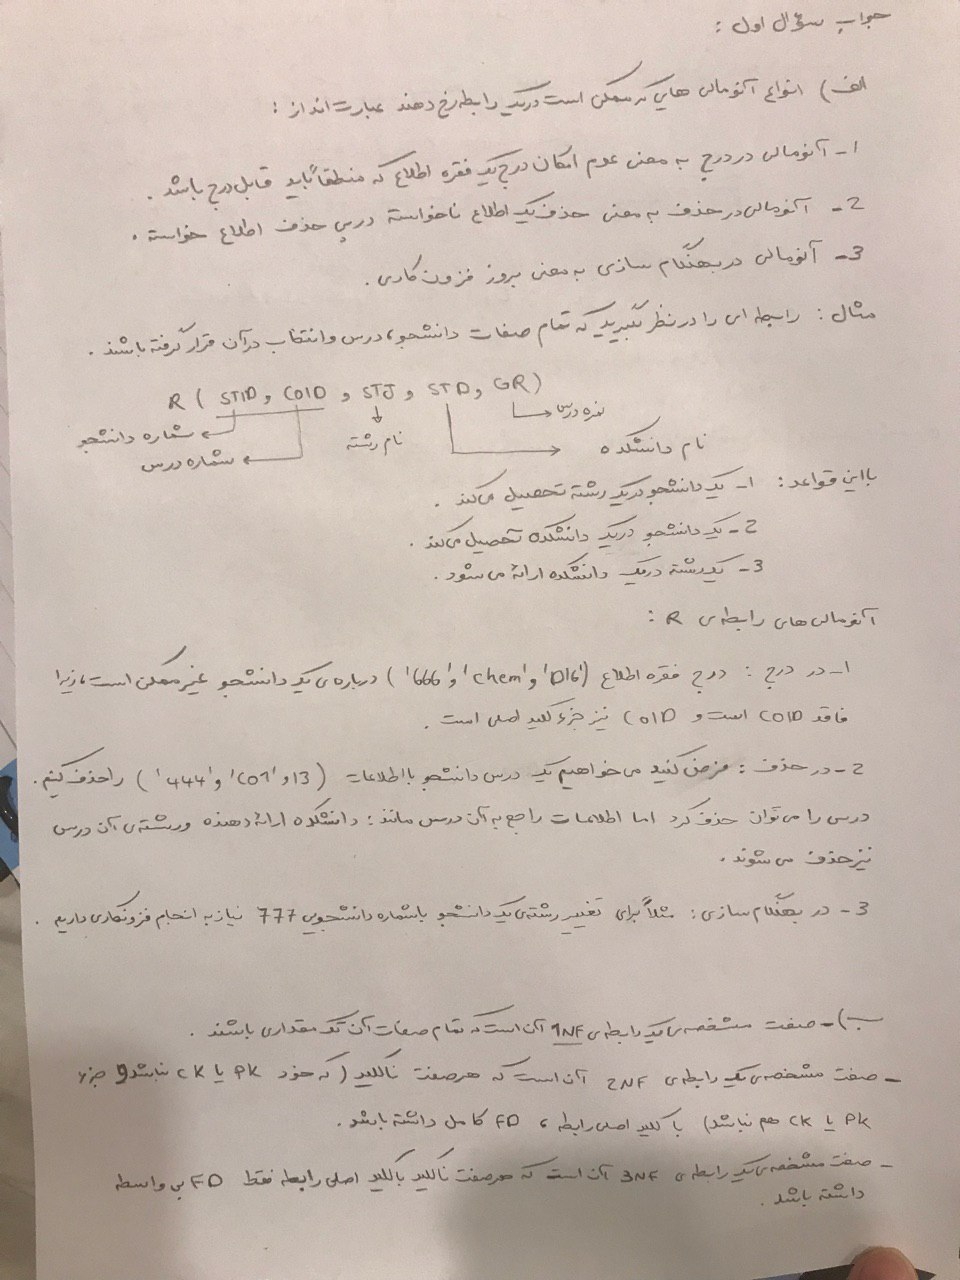
\includegraphics[width=0.5\linewidth]{Q1_1}
				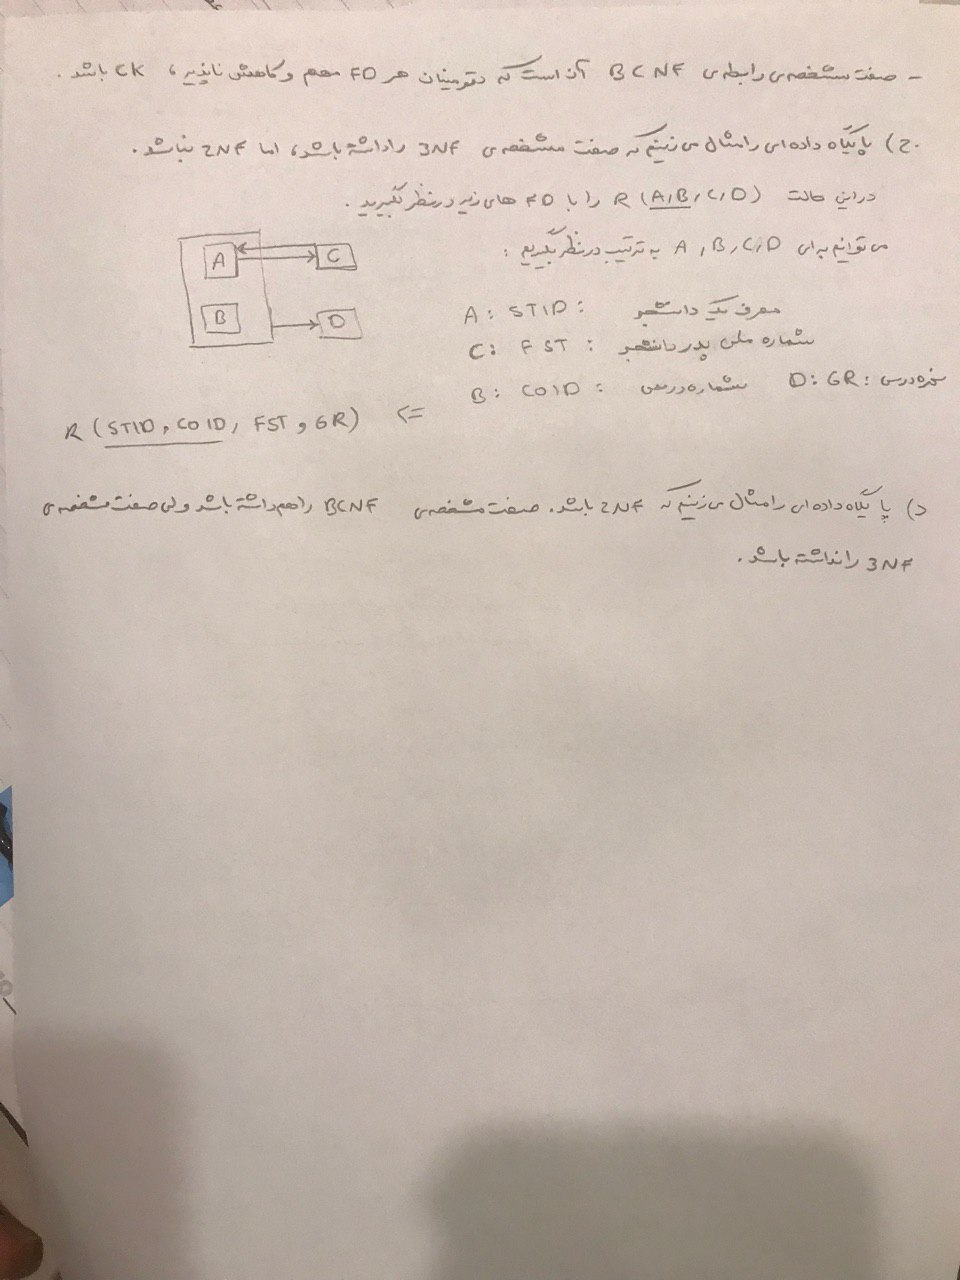
\includegraphics[width=1\linewidth]{Q1_2}  
	\end{center}

\section*{سوال دوم }
\subsection*{الف}
با توجه به قواعد معنایی می توان نتیجه گرفت که صفات 
\lr{PJNAME , PJMGRID , PJEMPNAME}
کلید های این جدول هستند بنابراین وابستگی ها به شرح زیر می باشد  : 
\begin{flushleft}
	\begin{enumerate}
		\item 
		\lr{PJNAME $\rightarrow$ PJMGRID}
		\item
		\lr{PJMGRID $\rightarrow$ PJNAME}
		\item 
		\lr{PJNAME $\rightarrow$ PJBUDGET}
		\item 
		\lr{PJNAME $\rightarrow$ PJSTARTDATE}
		\item 
		\lr{(PJNAME , PJMGRID , PJEMPID) $\rightarrow$ EMPRATING}
		\item 
		\lr{(PNAME , PJEMPID) $\rightarrow$ EMPSALARY}	
		\item 
		\lr{PJEMPID  $\rightarrow$ PJEMPNAME}
	\end{enumerate}
\end{flushleft}
\subsection*{ب}
با توجه به وابستگی های گفته شده در قسمت قبل نمودار 
\lr{FD}
آن به صورت زیر می باشد  : 
\begin{center}
		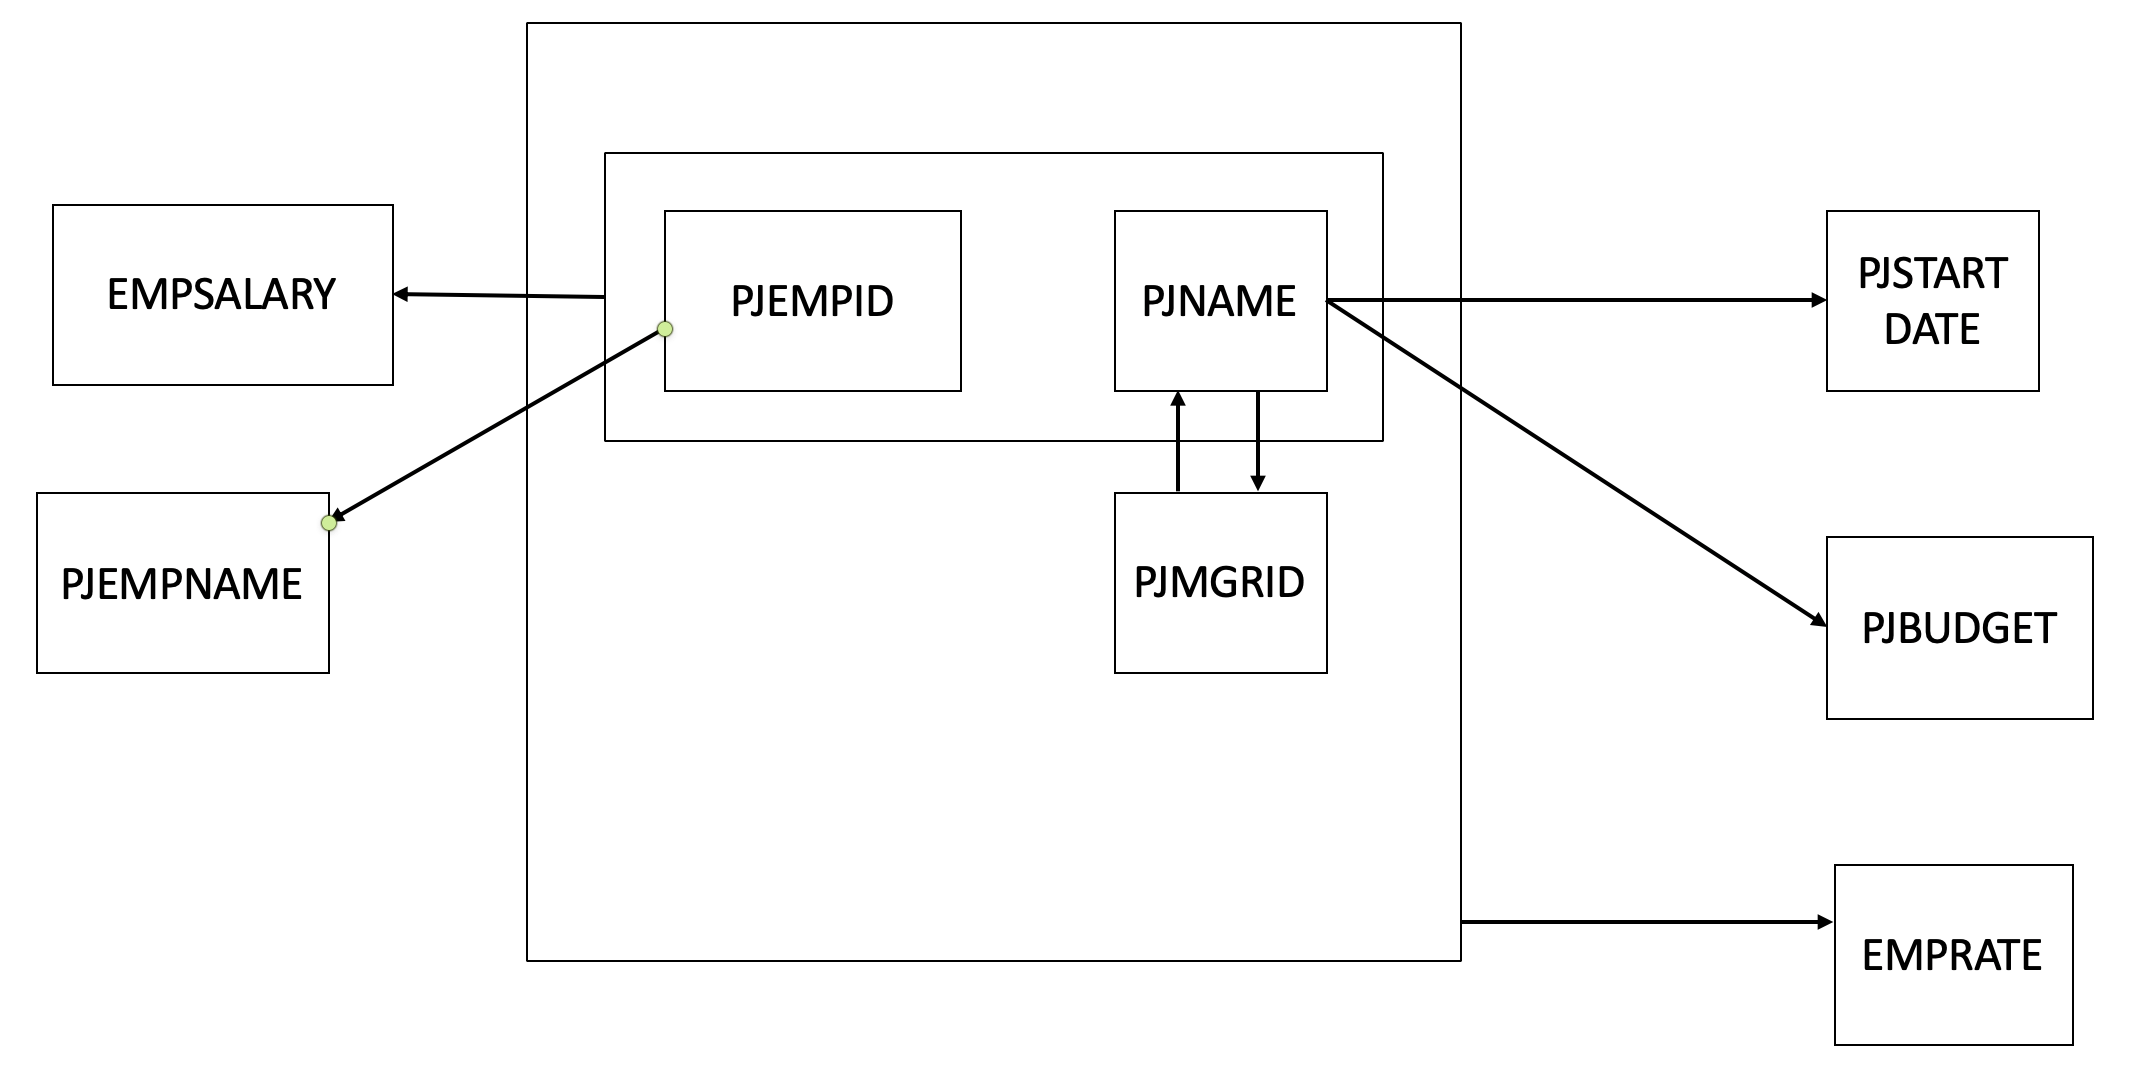
\includegraphics[width=.5\linewidth]{q2p1} 
\end{center}
با توجه به وابستگی های تابعی فرم نرمال 
\lr{BCNF}
به صورت زیر می باشد   : 
\\
\lr{PJEMP(PJNAME , PJEMPID)}
که هر دوی این صفات کلید خارجی می باشد و هر دو اجزا کلید اصلی هستند که 
\lr{PJEMPID}
کلید خارجی از رابطه 
\lr{EMP(PJEMPID , PJEMPNAME)}
می باشد  . 
\\
و کلید 
\lr{PJNAME}
یک کلید خارجی 
از رابطه 
\lr{PJ(PJNAME , PJMGRID , PJBUDGET , PJSTARTDATE)}
\\
و یک رابطه به صورت 
\lr{SALARY(PJNAME , PJEMPID)}
\\
و یک رابطه به صورت 
\lr{RATE(PJNAME , PJEMPID  , PJMGRID)}
\\
\hrule
\section*{سوال سوم }
\subsection*{الف}



\end{document}